\documentclass{sig-alternate}
 
\usepackage{color}
\usepackage{datetime}
\usepackage{graphicx}
\usepackage[shortlabels]{enumitem}
\usepackage{pifont}								% To get symbols for application table 																					overview

\newcommand{\TODO}[1]{{\small\bf \textcolor{red}{[TODO: #1]}}}
\newcommand{\thead}[1]{\textit{\tiny #1}}
\newcommand{\yes}{\checkmark}%
\newcommand{\no}{-}%
\newcommand{\cond}{(\checkmark)}%

\def\ms{\mathrm{ms}}

\begin{document}

\title{Icecite: A fully web-based research paper manager.}
%\title{Icecite: Draft}
\numberofauthors{1}
\author{
\alignauthor
Hannah Bast, Claudius Korzen\\[1mm]
%{(Note: names are in alphabetical order)}\\[1mm]
       \affaddr{Department of Computer Science}\\
       \affaddr{University of Freiburg}\\
       \affaddr{79110 Freiburg, Germany}\\
       \email{\{bast, korzen\}@informatik.uni-freiburg.de}
\date{\today, \currenttime}
}
\maketitle

\begin{abstract}
Some impressive abstract.
Process of identifying metadata and references is splitted into extraction and matching.
%We present \textit{Icecite}, a fully web-based and easy-to-use research paper management application. The aim of our application is to avoid the common, but usually bothersome tasks of a scientific research process. By offering the ability to manage, to read, to annotate, to share and to find scientific research papers easily, our application improves researchers daily working routine significantly. 
%
%In this paper, we will describe the overall design of Icecite and the basic ideas for each of the provided features. We present several results of our user-study, that we have performed to get an idea of users experience about Icecite. 
\end{abstract}
\section{Introduction}
Literature research is one of the most essential task to accomplish in a regular scientific research process. However, it's usually a complex and time-consuming task. That's why we have implemented \textit{Icecite}, a fully web-based research manager aimed to automatize and to facilitate the necessary steps of a \textit{digital} literature research process. \textit{Digital} means that Icecite concentrates on managing digital literary materials, namely scientific research papers provided as PDF files.

One of the core features of Icecite is the automatic identification of both, the metadata (title, author(s), year, journal, etc.) and the bibliographic references in given research papers. Our approach splits the identification process into 2 steps. In the first step, we extract significant data from given PDF files (e.g. the titles and the entries of bibliographies). In the second step, we match each extract to the referred record of an underlying digital library (e.g. DBLP or Medline) to get the full and correct metadata fields. Our approach outperforms traditional machine learning approaches in terms of runtime and accuracy of identified data.

On the basis of the automatic identification of data, Icecite can provide an extensive set of further features, that exceeds the feature sets of existing (mainly desktop-based) software solutions.  The full feature set of Icecite includes: 
\begin{enumerate}[{(1)}]
 \setlength{\itemsep}{-2pt}
 \item Managing research papers in a personal library.
 \item Automatic identification of metadata of research papers.
 \item Automatic identification of bibliographic references of research papers.
 \item Instant search in DBLP and Medline.  
 \item Instant (fulltext-)search in personal collection of research
 papers.
 \item Importing document from digital libraries into the library with a single click.
 \item Automatic search for PDF files, providing fulltexts of research papers.
 \item Reading \& Annotating of PDF files in browser.
 \item Tagging of  research papers with keywords.
 \item Offline usability.
 \item Synchronization of the library data (metadata, references, PDF files, annotations).
 \item Sharing of the library data with other member nearly in real-time.
 \item Fully web-based and easy-to-use user interface
\end{enumerate}
In the following, we will give an overview how the listed features act together to form the general structure of Icecite and how they support the following most essential tasks of a proper literature research process.
%Each listed feature contributes to improve the experiences on doing literature research. To substantiate this, we now introduce the most essential tasks of a proper literature research process and clarify, how they are automatized by Icecite.

\paragraph{Organize collections of research papers} 
\noindent
Doing scientific literature research usually implies the need to manage a set of collected literary materials, i.e. digital research papers provided as PDF files as mentioned above.

The collection may consist of locally stored files or bookmarks to the locations of files in web, or both. Depending on the size of the collection, keeping a consistent structure on naming the files are recommended, in order to keep track of them. However, finding proper filenames and renaming the files are annoying and time-consuming tasks. 

\begin{figure*}[!ht]
  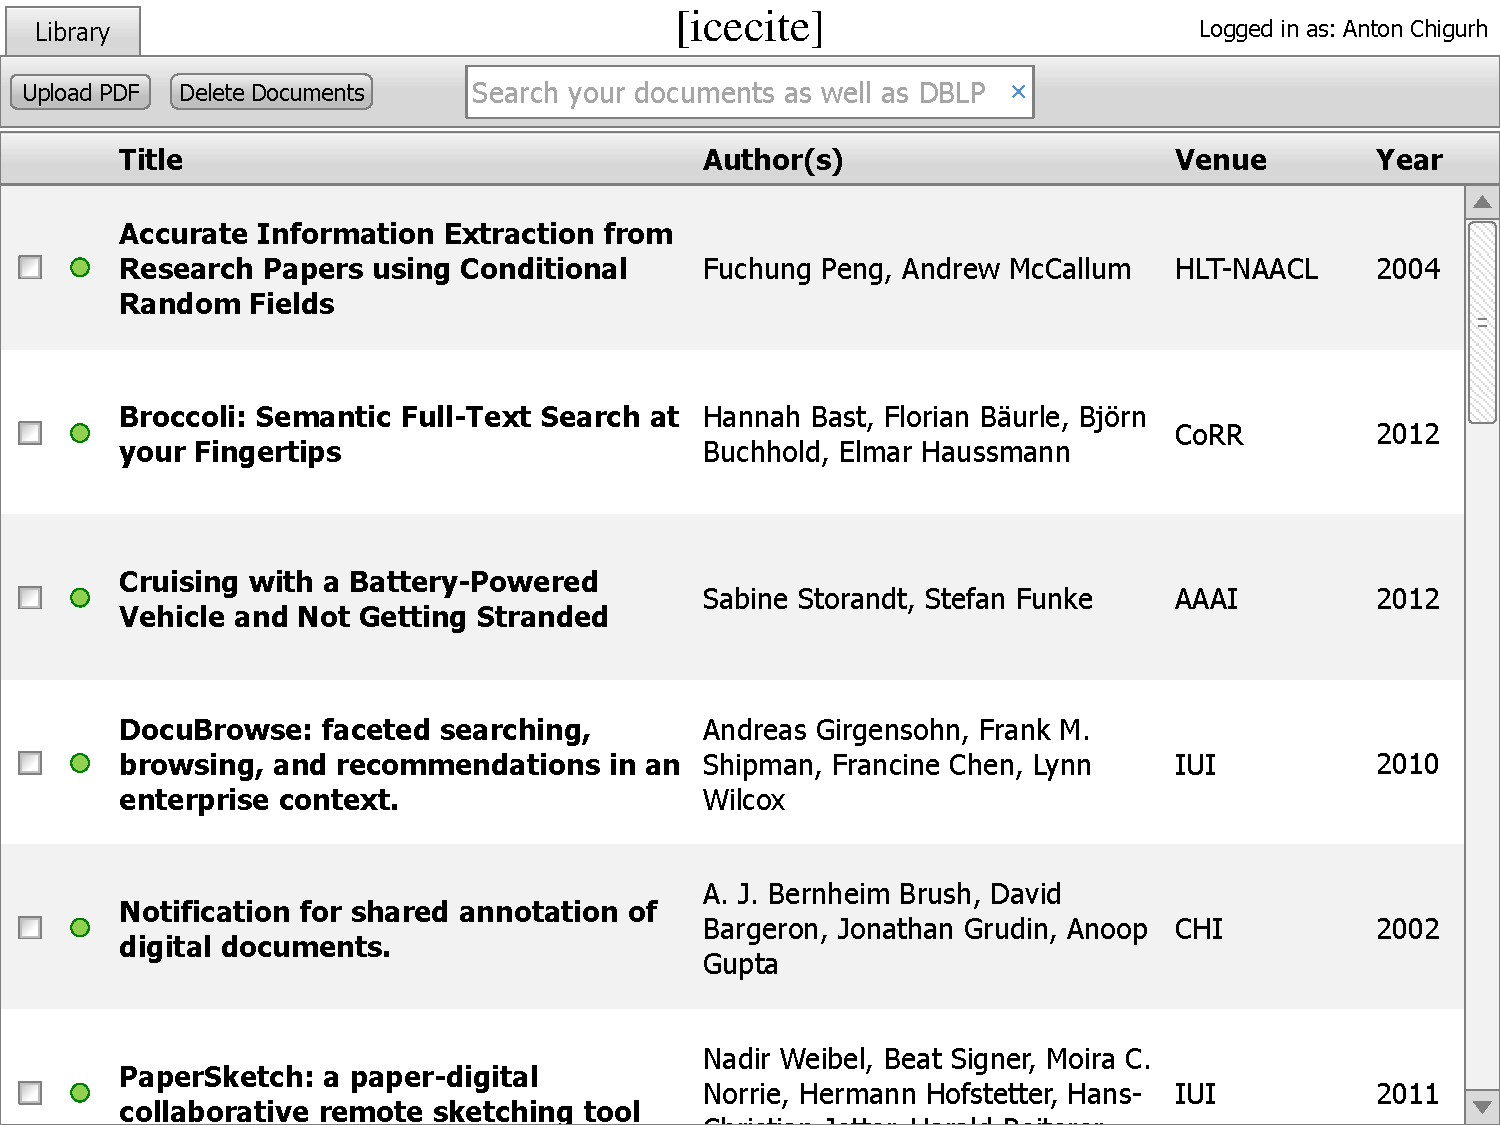
\includegraphics[width=\textwidth]{./figures/libraryview}
  \caption{A screenshot of the \textit{library view} in Icecite. Each entry of library is listed with the following metadata fields: title, author(s), conference and year of publication. The checkbox besides each entry exists, to select the entry for deletion (the deletion is actually done by clicking the button \textit{Delete Documents} in the upper left).  The small bullet to the left of the title of each entry displays the status of entry (a \textit{green} bullet means, that the full metadata were found for entry). On clicking the button \textit{Upload PDF}, you can add a locally stored PDF file to library. The needed metadata will be computed automatically then. You can type in a search query into the search field (located to the right of the \textit{Delete Document} button), to search in own library as well as in the digital library \textit{DBLP}. On clicking an entry of search result, it will be added to library. In contrast, on clicking an entry of library, user is forwarded to the \textit{document view} (cf. Figure \ref{fig:screenshot_documentview}).}
  \label{fig:screenshot_libraryview}
\end{figure*}

Icecite eliminates these steps entirely by holding all the collected research papers (\textit{documents}) in a personal \textit{library}. A library is placed in the \textit{library view} of Icecite (shown in figure \ref{fig:screenshot_libraryview}, consider the caption below the figure for a detailed explanation of each UI-element). On adding a document to the library, its metadata and its bibliographic references are identified automatically due to the features (1)+(2). Because the metadata are used to describe the document uniquely, there is no need anymore to name files manually. The identified references of a document are placed next to the PDF file in the \textit{document view} (shown in figure \ref{fig:screenshot_documentview}), that is accessible via clicking a document in the library view. A more detailed discussion about our approach of automatic identification of metadata and bibliographic references can be found in section \ref{sec:extraction}.    

Although Icecite is web-based, all library data (metadata, PDF files, etc.) are stored locally on client's filesystem. That's why some features of Icecite can be used even in case of offline mode, e.g. browsing the library, annotating PDF files or load PDF files into the library (certainly without automatic identification of metadata and references). It can be achieved by using features of the html5 standard, as described in section \ref{sec:html5}.	

Additionally, the library data are synchronized periodically with the server to (1) access them from any location and (2) share them with other users for collaboration. The mechanism of data synchronization is described in section \ref{sec:sync}.

\begin{figure*}[ht]
  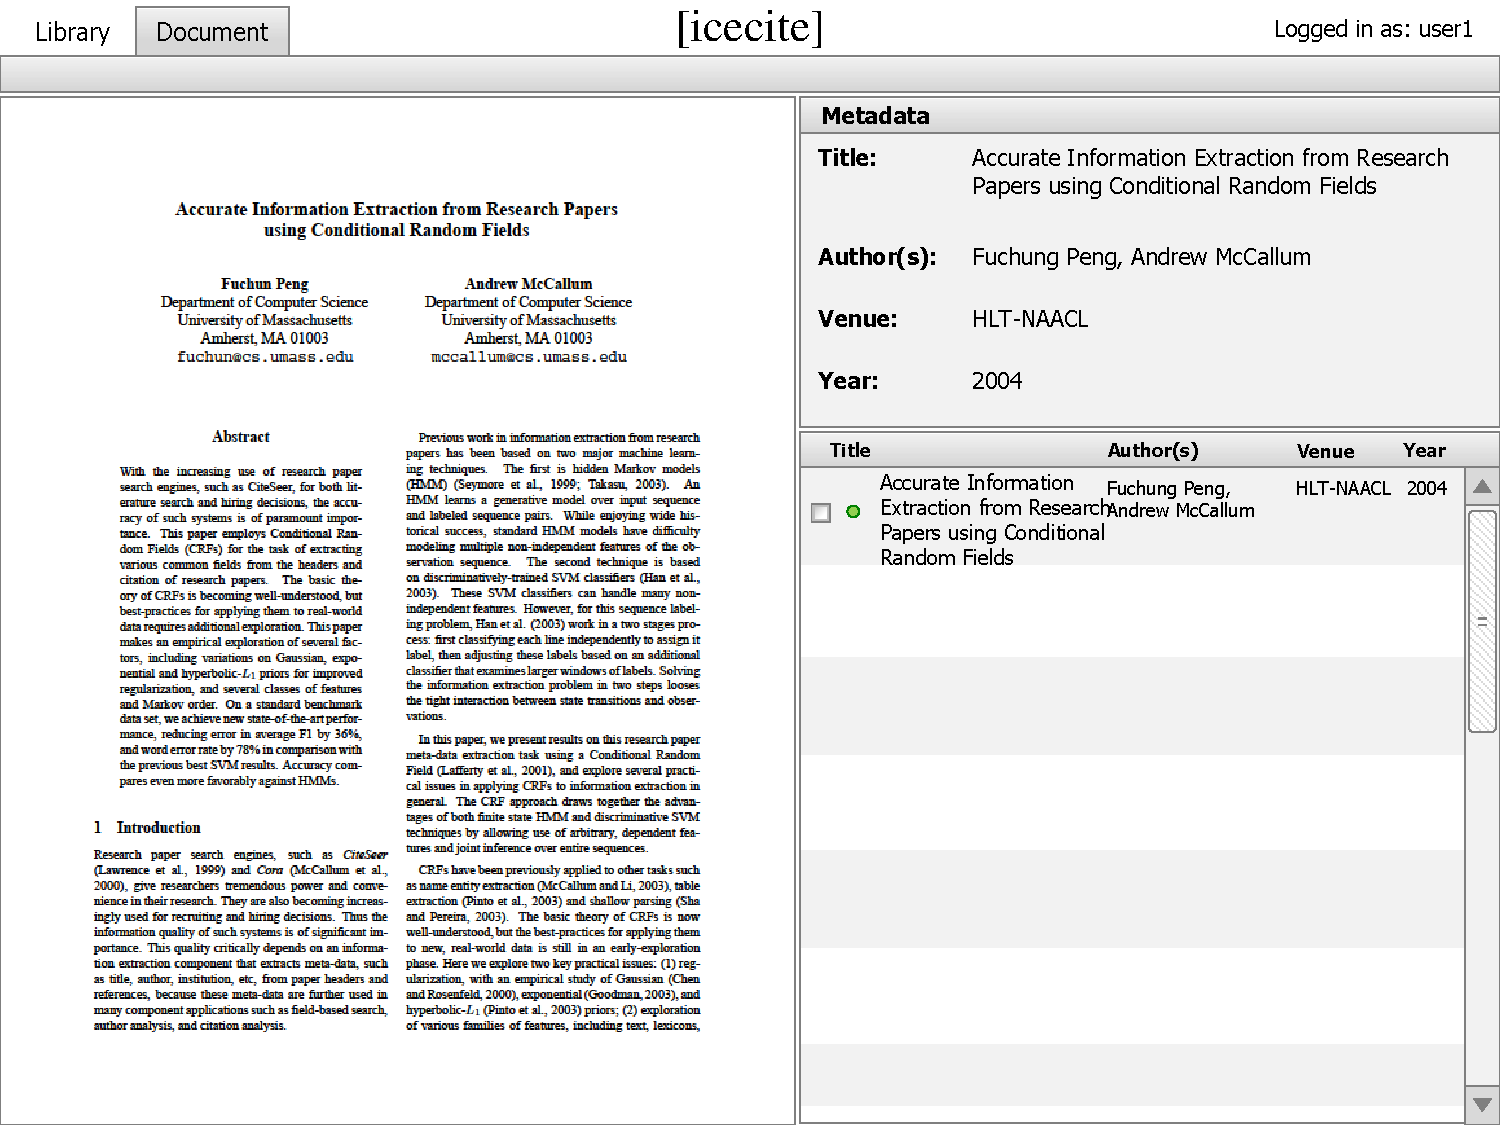
\includegraphics[width=\textwidth]{./figures/documentview}
  \caption{A screenshot of the \textit{document view} in Icecite. It shows both, the pdf file of research paper and the metadata of the paper and its references. Here you can read, annotate and comment the pdf file (you can turn the pdf into fullscreen-mode to hide the metadata to the right) and study the metadata of references. The entries of references list are of the same design as the entries in the \textit{library view} (cf. figure \ref{fig:screenshot_libraryview}). Again, on clicking an entry of references, you can add it to library, to read, annotate and share it and to study its references.}
  \label{fig:screenshot_documentview}
\end{figure*}

\paragraph{Searching for topic-related research papers} 
\noindent
In order to explore topic-related research papers and to extend the personal collection with them, generally the following 4 sources can be consulted:

\par\medskip\noindent
\textit{(S1)} Digital libraries, such as \textit{DBLP} or \textit{Medline}.
\par\smallskip\noindent
\textit{(S2)} The web, such as publisher websites (like \textit{ACM}, \textit{IEEE}, \textit{Springerlink}, etc.)
\par\smallskip\noindent
\textit{(S3)} Bibliographies from already known research papers.
\par\smallskip\noindent
\textit{(S4)} Personal recommendations.
\medskip

The listed sources differ from each other in the amount of provided data. While the sources \textit{(S1)} and \textit{(S2)} may provide (links to) PDF files of research papers, the sources \textit{(S3)} and \textit{(S4)} usually don't (but only parts of metadata fields). Hence, in case of sources \textit{(S3)} and \textit{(S4)}, extra effort is needed to retrieve the PDF files (e.g. by consulting the source \textit{(S1)} or \textit{(S2)} in addition). However, the invested time and effort may be in vain, if a file isn't fetchable, because it isn't available in general or the access to it is restricted and only available to licensees. 

Due to the automatic identification of bibliographic references (2), the instant search in DBLP and Medline (3) and the automatic search for PDF files (5), Icecite speeds up the whole process of fetching topic-related research papers substantially. 
\TODO{Eliminate this listing, and reuse it in infrastructure section} 
Generally, there are three ways to add a new document to the library: 

\par\medskip\noindent
\textit{(ADD 1)} Upload a PDF file to the library.
\par\medskip\noindent
\textit{(ADD 2)} Click an entry in the reference list of a selected document in the document view.
\par\medskip\noindent
\textit{(ADD 3)} Type a search query into the search field of the library view to browse for any entries in a digital library (DBLP or Medline). Click a record of the search result.
\medskip

Variant \textit{(ADD 1)} is followed directly by the automatic identification of the metadata and the bibliographic references of the research paper given by the uploaded PDF file. Once all the metadata and references are retrieved, the document is added to the library.

In contrast, variants \textit{(ADD 2)} and \textit{(ADD 3)} are firstly followed by the automatic search for a PDF file, that contains the fulltext of the clicked record in the references list (resp. the search result). The PDF file is located in the web via the metadata, which were retrieved on the references identification (resp. via the metadata provided by the digital library). Once the PDF file was found, the further processing is similar to that for variant \textit{(ADD 1)} as described above. See section \ref{sec:search} for a more detailed discussion of the search in digital libraries and the automatic search for PDF files.

\paragraph{Reading research papers} 
\noindent
While reading the PDF file of a research paper, it's quite common, to highlight some text passages and to make some notes to it. With Icecite, PDF files can be read online, if there is a proper browser plugin is installed to display the PDF files in the browser and can be even annotated, if the plugin of Adobe Acrobat is used. On implementing this feature, we have paid attention to use \textit{native}\footnote{With native annotations we mean those annotations, which conform to the official PDF specifications} annotations. This ensures, that the annotations are identified as such not only within Icecite, but also in various external PDF viewers. See the detailed desciption of this feature in section \ref{sec:annotations}, why this intention isn't trivial to achieve.

\paragraph{Collaborate in groups} 
\noindent
On collaborating in (research-)groups to review some research papers together, many individual annotations are produced. Icecite is able to combine the individual annotations made to a PDF file to get a general conclusion. The data of library can be shared with other users nearly in real-time. So, once the set of documents and annotations in shared libraries was changed by a member of group, the changes are displayed to the other members instantly. See section \ref{sec:sync} for a more detailed discussion of this feature. \\

In section \ref{sec:related_work}, we will introduce some applications, that are related to Icecite. There are both, desktop-based and web-based applications, although existing desktop-based applications typically provide larger feature sets than existing web-based applications. We will compare the features of both types with those of Icecite.
However, desktop-applications have some drawbacks... \\
\TODO{list drawbacks of desktop applications.}\\
\TODO{Present results of experiments}.\\
\TODO{Present results of user study}.

At the end of this introduction, we want to clarify, that the contribution of this paper is the overall design of Icecite and the basic ideas for each of the individual components of the system. Consider, that these components are complex problems each on their own and can not be discussed in all details in this paper. However, in section \ref{sec:futurework} we will give you an idea, how the various components can be optimized on future research.
\section{Related Work}\label{sec:related_work}
We split the related work section mainly in three parts. In the first part, we introduce existing \textit{desktop-based} and \textit{web-based applications} similar to Icecite. In the second part, we focus on existing \textit{extraction techniques} to retrieve informations about the metadata and/or the bibliographic references from research papers. 
Because we use a metadata knowledge base in background and match an extract to the referred record in the knowledge base to get full and correct metadata, we finally focus in the third part on \textit{record matching techniques}.

\subsection{Related Applications}
A lot of applications were already developed, aimed to support researchers during a literature research process. In this section, we introduce some of them and compare their feature sets. Table \ref{tab:featureoverview} summarizes the individual feature sets in an overview.  

\subsubsection{Desktop-based Applications}
The upper part of Table \ref{tab:featureoverview} breaks down the provided features of \textit{desktop-based} applications. All of them can be seen as \textit{research managers} and are quite similar regarding to their basic structure: research paper are manageable in individual libraries, where they are listed with their (usually automatically identified) metadata. However further features differ from application to application. Because we can't describe all applications in detail here, we pick a single representative one, namely \textit{Mendeley} \cite{www:mendeley}. We have chosen Mendeley, because it considers itself to be "the world's largest social reference management system" \cite{DBLP:conf/www/KrakerKJG12}. Moreover we believe that its feature set comes closest to the features of a state-of-the-art research manager.
In the following, we will examine Mendeley's feature set in detail and compare it with those of the other applications.  

%\begin{table*}[!ht]
%\centering
%\renewcommand{\arraystretch}{1.3}
%\setlength{\tabcolsep}{1pt}
%\begin{tabular}{l|cccccccccccccccc}
%\textit{Name of application }	& \thead{(WEB)} & \thead{(EX-M)} & \thead{(EX-R)} & \thead{(PDF)} & \thead{(ANN)} & \thead{(TAG)} & \thead{(S-PL)} & \thead{(S-FT)} & \thead{(S-DL)} & \thead{(IMP-DL)} & \thead{(IMP-R)} & \thead{(RES-PDF)} & \thead{(SY-M)} & \thead{(SY-P)} & \thead{(SY-A)} & \thead{(SH)}\\ \hline
%Citavi \cite{www:citavi} 			& \no & \cond & \no & \yes & \no & \yes & \yes & \no & \yes & \yes & \no & \cond & \no & \no & \no & \cond   \\
%EndNote \cite{www:endnote} 		& \no & ? & ? & ? & ? & ? & ? & ? & ? & ? & ? & ? & ? & ? & ? & ? \\
%EverNote \cite{www:evernote}	& \cond & \no & \no & \yes & \no & \yes & \yes & \yes & \no & \no & \no & \no & \yes & \yes & \no & \yes \\
%Mendeley \cite{www:mendeley}	& \cond  & \yes & \no & \yes & \yes & \yes & \yes & \yes & \no & \cond  & \no & \no & \yes & \yes & \yes & \yes  \\
%Papers \cite{www:papers}			& \no & ? & ? & ? & ? & ? & ? & ? & ? & ? & ? & ? & ? & ? & ? & ? \\
%Qiqqa \cite{www:qiqqa}				&	\cond & \yes & \no & \yes & \yes & \yes & \yes & \yes & \yes & \yes & \no & \no & \yes & \yes & ? & \yes \\
%ReadCube \cite{www:readcube} 	& \no & \yes & \cond & \yes & \yes & \no & \yes & \yes & \yes & \yes & \cond & \yes & \no & \no & \no & \no  \\
%Zotero \cite{www:zotero}			& \cond & \yes & \no & \yes & \no & \yes & \yes & \no & \no & \yes & \no & \no & \yes & \yes & \no & \yes \\ \hline
%BibSonomy \cite{www:bibsonomy}& \yes & \no & \no & \yes & \no & \no & \yes & \no & \yes & \yes & \no & \no & \no & \no & \no & \yes \\
%CiteULike \cite{www:citeulike}& \yes & \no & \no & \yes & \cond & \yes & \yes & \yes & \yes & \yes & \no & \no & \no & \no & \no & \yes\\
%EndNote Web \cite{www:endnoteweb} & \yes & \no & \no & \no & \no & \yes & \yes & \no & \yes & \yes & \no & \no & \no & \no & \no & \yes \\
%RefWorks \cite{www:refworks} 	& \yes & \no & \no & \no & \no & \no & \yes & \no & \yes & \yes & \no & \no & \no & \no & \no & \yes \\
%A.nnotate \cite{www:annotate}	& \yes & \no & \no & \yes & \yes & \yes & \yes & \no & \no & \no & \no & \no & \no & \no & \no & \yes \\
%Crocodoc Personal \cite{www:crocodoc}	& \yes & \no & \no & \yes & \yes & \no & \no & \no & \no & \no & \no & \no & \no & \no & \no & \yes \\
%WebNotes \cite{www:webnotes}	& \yes & \no & \no & \yes & \yes & \yes & \yes & \yes & \no & \no & \no & \no & \no & \no & \no & \yes \\
%\end{tabular}
%\caption{Overview of the provided features by applications related to Icecite. If a feature is fully provided by an application, it's labeled with an checkmark. If a feature is only partially provided, it's labeled with an circle. The upper part of the table denotes desktop-based, the lower part web-badsed applications. Each acronym in the header of the table denotes an specific feature. The meanings of them are as follows: \textit{(WEB)}: application is web-based; \textit{(EX-M)}: extraction of metadata from PDF files; \textit{(EX-R)}: extraction of references from PDF file; \textit{(PDF)}: management of PDF files; \textit{(ANN)}: annotating PDF files; \textit{(TAG)}: tagging documents in the personal library; \textit{(S-PL)}: searching the personal library; \textit{(S-FT)}: searching the fulltexts; \textit{(S-ES)}: searching in external sources; \textit{(IMP-ES)}: Importing documents from external sources into personal library; \textit{(IMP-R)}: Importing referenced documents into the personal library; \textit{(RES-PDF)}: resolving PDF files for external documents; \textit{(SY-M)}: Synchronization of metadata; \textit{(SY-P)}: Synchronization of PDF files; \textit{(SY-A)}: Synchronization of annotations; \textit{(SH)}: Sharing documents of personal library with other users.}
%\label{tab:featureoverview}
%\end{table*}

\begin{table*}[!ht]
\centering
\renewcommand{\arraystretch}{1.3}
\setlength{\tabcolsep}{1pt}
\begin{tabular}{l|cccccccc}
\textit{Name of application }	& \thead{(CLOUD)} & \thead{(OFFLINE)} & \thead{(SHARED)} & \thead{(EX-M)} & \thead{(EX-R)} & \thead{(AUTO-DL)} & \thead{(ANNOT)} & \thead{(SEARCH)} \\ \hline
Citavi \cite{www:citavi} 			& \no & \yes & \cond & \cond & \no & \cond & \no & \cond \\
EndNote \cite{www:endnote} 		& ? & ? & ? & ? & ? & ? & ? & ? \\
EverNote \cite{www:evernote}	& \yes & \yes & \yes & \no & \no & \no & \no & \cond \\
Mendeley \cite{www:mendeley}	& \yes & \yes & \yes & \yes & \no & \no & \yes & \cond \\
Papers \cite{www:papers}			& ? & ? & ? & ? & ? & ? & ? & ? \\
Qiqqa \cite{www:qiqqa}				&	\yes & \yes & \yes & \yes & \no & \no & \yes & \yes  \\
ReadCube \cite{www:readcube} 	& \no & \yes & \no & \yes & \cond & \yes & \yes & \yes  \\
Zotero \cite{www:zotero}			& \yes & \yes & \yes & \yes & \no & \no & \no & \cond \\ \hline
BibSonomy \cite{www:bibsonomy}& \yes & \no & \yes & \no & \no & \no & \no & \no \\
CiteULike \cite{www:citeulike}& \yes & \no & \yes & \no & \no & \no & \cond & \yes \\
EndNote Web \cite{www:endnoteweb} & \yes & \no & \yes & \no & \no & \no & \no & \cond \\
RefWorks \cite{www:refworks} 	& \yes & \no & \yes & \no & \no & \no & \no & \cond \\
A.nnotate \cite{www:annotate}	& \yes & \no & \yes & \no & \no & \no & \yes & \cond \\
Crocodoc Personal \cite{www:crocodoc}	& \yes & \no & \yes & \no & \no & \no & \yes & \no \\
WebNotes \cite{www:webnotes}	& \yes & \no & \yes & \no & \no & \no & \yes & \cond \\
\textbf{Icecite} 							& \yes & \yes & \yes & \yes & \yes & \yes & \yes & \yes \\
\end{tabular}
\caption{Overview of the provided features by applications related to Icecite. If a feature is fully provided by an application, it's labeled with an checkmark. If a feature is only partially provided, it's labeled with an circle. The upper part of the table denotes desktop-based, the lower part web-badsed applications. Each acronym in the header of the table denotes an specific feature. The meanings of them are as follows: \textit{(WEB)}: application is web-based; \textit{(EX-M)}: extraction of metadata from PDF files; \textit{(EX-R)}: extraction of references from PDF file; \textit{(PDF)}: management of PDF files; \textit{(ANN)}: annotating PDF files; \textit{(TAG)}: tagging documents in the personal library; \textit{(S-PL)}: searching the personal library; \textit{(S-FT)}: searching the fulltexts; \textit{(S-ES)}: searching in external sources; \textit{(IMP-ES)}: Importing documents from external sources into personal library; \textit{(IMP-R)}: Importing referenced documents into the personal library; \textit{(RES-PDF)}: resolving PDF files for external documents; \textit{(SY-M)}: Synchronization of metadata; \textit{(SY-P)}: Synchronization of PDF files; \textit{(SY-A)}: Synchronization of annotations; \textit{(SH)}: Sharing documents of personal library with other users.}
\label{tab:featureoverview}
\end{table*}


Mendeley is basically a desktop-based application. Though Mendeley comes with a web-interface to browse and manage the library data in an ordinary web browser, which were synchronized with Mendeley's server. However the number of features of the web interface is restricted and that's why there is a '\cond' in first column of Table \ref{tab:featureoverview} for Mendeley (a similar argument is valid for EverNote and Qiqqa). Further, Zotero comes with an extension for the Firefox browser.
 
In Mendeley, the metadata of research papers are extracted automatically from the PDF file. In contrast, the extraction of bibliographic references from PDF files isn't provided, neither in Mendeley\footnote{Consider, that the extraction of references was supported in a previous version of Mendeley, but was removed again, "because it was consuming a fair amount of resources (on client and server side) without providing enough value" \TODO{How to cite the referred blog post?}} nor in other research managers. Consider, that ReadCube provides a feature called \textit{enhancing PDF files}. For example, this feature enhance particular PDF files with prepared informations about bibliographic references. However, ReadCube doesn't extract these data directly from PDF files, but tries to resolve the DOI (digital object identifier) of a document and gathers the data from any web pages afterwards. Hence prepared references are only available, when the document contains such a DOI and when the data are retrievable from the web.

Further features of Mendeley are the built-in PDF viewer to read and to annotate PDF files within the application and the chance to tag documents with specific keywords. All data including the fulltexts of documents can be searched to find particular entries in the library. However external sources (like digital libraries) aren't browseable within Mendeley, as it is possible within Citavi, Qiqqa and ReadCube.  

Furthermore, a bookmarklet (the so called \textit{Web importer}) can be installed to the ordinary web browser to import the metadata of research papers from several external sources into the personal library, along with the corresponding PDF file, if it's provided by the chosen source. But the weaknesses of this feature are (1) the need to switch between Mendeley's interface and the browser and (2) the lack of an automatic search for PDF files in case that the external source doesn't provide PDF files. In contrast, ReadCube searches for PDF files on browsing the external sources to import them into the library with a single click. If a PDF could be \textit{enhanced} (see above), this feature is also used to import a reference along with its PDF file into the library easily. However the approach to import documents by references is very simplistic, because the retrieved reference string can be just sent to an external source as query, in the hope that the correct record will be found in the external source.

As mentioned above, Mendeley can synchronize the library data with its server to access them via the provided web interface or from several local installations of Mendeley on various devices. Moreover, the data synchronization offers the chance to share them with other members of individual groups to collaborate.

\TODO{Explain some special features? For example the feature of ReadCube: list all citing papers} 

\subsubsection{Web-based Applications}
The lower part of Table \ref{tab:featureoverview} breaks down the provided features of \textit{web-based} applications. Compared to desktop-based applications, their amount is usually much smaller. Most of the web-based applications focus only on specific subareas of literature research, like \textit{pure metadata managing} or \textit{PDF file annotating}. 

Pure metadata managing is for example supported by \textit{BibSonomy}, \textit{CiteULike}, \textit{EndNote Web} and\textit{RefWorks} \cite{www:refworks}. Basically, each application allows to collect bibliographic metadata systematically in a personal library and to generate bibliographies for own publications from them. A record can be either created manually or imported from external sources. All metadata records are generally fully searchable. Furthermore, libraries are typically shareable with other users to get a combined set of metadata. Two of the listed applications (namely BibSonomy and CiteULike) allow to attach PDF files to each record, whereas the automatic extraction of metadata and references is generally not supported. Further, annotating PDF files is possible seldomly because only CiteULike provides this feature in a premium version for paying users. Though, annotating PDF files in the browser is the aim of the following type of web-based applications.
 
Annotating PDF file in the browser is for example supported by \textit{A.nnotate}, \textit{Crocodoc} or \textit{WebNotes}. All applications allow to read, annotate and comment PDF files collaboratively. The features are usable via an ordinary web browser due to techniques of HTML5 or Flash. Basically, the scopes of supported files are not limited to PDF files, but also include arbitrary text files, images and even websites. Hence, such applications are not primarily intended to support a literature research process. That's why features like \textit{automatic metadata extraction from PDF files} or \textit{automatic search for fulltexts} are usually missing in annotation applications \\

\subsubsection{Comparison of web-based and desktop-based applications}
\TODO{Wrote something about our aim, e.g. providing same scope of features, that are currently provided by desktop-based applications}.
%We have seen that a lot of features were already implemented, aimed to automatize parts of the literature research process. However, we think that there is still room for more supporting features. For example, there is no application, that provides a feature to identify the metadata of the references of research papers, although they offer a great potential to find related papers. 

%\TODO{More missing features}.
%\TODO{Explain the weakness of approaches of existing applications}. 

\subsection{Metadata Extraction Techniques}
In this section, we focus on related techniques to extract the metadata fields (title, author(s), affiliation(s), journal, etc.) of research papers and their bibliographic references. At first we will introduce some machine learning techniques, namely \textit{Hidden Markov Models}, \textit{Support Vector Machines} and \textit{Conditional Random Fields} and analyze their extraction accuracy. Afterwards, we will do the same with rule-based techniques 
% and examine, which techniques are used by the applications introduced above.

\subsubsection{Hidden Markov Models (HMMs)}
Hidden Markov Models have been applied to identify the metadata fields of both, research papers and their references. Seymore et al   \cite{Seymore99LearningHMM} describe an approach, where a manually-constructed model are used to identify the metadata fields in the headers of research papers. The constructed model contains multiple states per field. They achieve an extraction accuracy of 92.9\% over all metadata fields. 

Borkar et al \cite{DBLP:conf/sigmod/BorkarDS01} use a nested HMM to identify the metadata fields of references. The constructed HMM contains one state per metadata field. Each state itself consists of another HMM, representing the internal structure of the field. With this method, Borkar et al achieve an average precision and recall ratio of 0.87 over all fields.

\subsubsection{Support Vector Machines (SVMs)}
Support Vector Machines are used by Han et al \cite{DBLP:conf/jcdl/HanGMZZF03} to identify the metadata fields in the headers of research papers. Their experiments based on 500 training headers and 435 test headers resulted in an overall accuracy of 92.9\%.

The metadata extraction of Mendeley relies on a two-stage SVM and is aimed to extract the title and the authors from research papers (Granitzer et al, \cite{DBLP:conf/sac/GranitzerHJK12}). In a first step, it classifies each line of the header text into title, author and other classes using text and formating features. In a second step, the classification is 
improved by using contextual information such as the predicted class labels of the neighboring lines. The experiments of Granitzer et al. based on a training set of 1000 research papers. They resulted in an average precision rate of 0.81 and an average recall rate of 0.62 for the author extraction and in an average precision rate of 0.94 and an average recall rate of 0.91 for the title extraction.

\subsubsection{Conditional Random Fields (CRFs)} 
Peng et al. \cite{DBLP:conf/naacl/PengM04} utilizes Conditional Random Fields to extract the metadata from both, the headers and the references of research papers. Experiments to test the field extraction from headers were performed on 500 training headers and 435 test headers and resulted in an overall accuracy of 73.3\%. Experiments to test the field extraction from references were performed on the \textit{Cora} dataset, containing 500 references. They resulted in an overall extraction accuracy of 77.3\%. \TODO{The claimed numbers are instance accuracies: the percentage of instances in which every word is correctly labeled. Word accuracies is quite higher} \\

Machine learning techniques are generally considered to be robust and adaptable \cite{DBLP:conf/jcdl/HanGMZZF03}. Moreover, the above announced extraction accuracies show, that utilizing machine learning techniques is a promising way to extract metadata from research papers and their references.

However as claimed by Guo and Jin \cite{DBLP:conf/pdcat/GuoJ11}, generating accurate labeled datasets needed to train the models is time-consuming and costly. Alternatives to machine-learning approaches are rule-based approaches, which are usually faster, but less accurate.

\subsubsection{Rule-based approaches}
Rule-based approaches base on a set of rules, describing how to identify the metadata to extract in research papers. The rules are deduced from human observations regarding the basic structures of research papers.

J�ran Beel et al. \cite{DBLP:conf/ercimdl/BeelGSF10} have identified the titles of 693 research papers by using a rule-based approach, i.e. by utilizing their layout informations, i.e. the font sizes and their positions within the documents. Their experiments yield to 77,9\% correctly identified titles.

Cortez et al \cite{DBLP:conf/jcdl/VilarinhoSGMM07} propose a unsupervised knowledge-based approach to recognize the components of reference strings given in any format. The authors split each reference string into blocks and label each block with the name of a metadata field. Therefore a knowledge is used, that was constructed automatically from an existing set of sample metadata records. Experiments were performed on 300 reference strings and have produced an overall extraction accuracy of 82\%. \TODO{Verify this accuracy}.

All approaches seen so far try to extract any metadata fields of research papers and/or their references without utilizing any metadata knowledge bases to guide the extraction process. Guo and Jin introduce this approach in \cite{DBLP:conf/pdcat/GuoJ11}. They extract metadata using a rule-based approach and check if there is any matched document in a knowledge base, which is mainly developed from DBLP. If matched, they use the metadata stored in the knowledge base to make sure the extracted reference metadata are correct. The experiments on 97 research papers and 2157 references to be extracted resulted in an average extraction accuracy of 89,1\% over all metadata fields.
 
Basically, our approach follows up the approach of Guo and Jin. In a first step, the title and each reference-string is extracted from a research paper, profiting from the speed advantage of a simple rule-based approach compared to a machine learning approach. In a second step, each extract is matched to a record of DBLP or Medline, to get full and correct metadata. That's why we inspect existing record matching techniques in the following.   

\subsection{Record Matching Techniques} \label{sec:relatedwork:recordmatching}
As described above, we match the extracted data to a record of a metadata knowledge base to get full and correct metadata. In this section, we inspect the most common record matching techniques.
   
For our purposes, record matching can be defined in the following way: Given an extract (i.e. the title or a reference of a research paper), that refer to a record in the metadata knowledge base. Identify this record and associate it with the given extract. The task may be affected by noisy factors (like extraction failures, different spellings, abbreviations, etc.), whereby the typographic design of a metadata field may differ from the specifications in the referred record. 

Most of the existing record matching techniques base on string comparison approaches, which generally determines the similarity of two strings on the base of character-based, token-based or phonetic-based similarity measures. We only focus on character-based measures here. For a detailed discussion of all the measures, see the surveys in \cite{DBLP:journals/tkde/ElmagarmidIV07} and \cite{DBLP:journals/cacm/KanT08}.

Character-based similarity measures analyzes the similarity of two given strings $s$ and $t$ by comparing the strings character by character. For example, the \textit{Levenshtein distance} \cite{levenshtein} between $s$ and $t$ is defined as the minimal number of needed edit operations (\textit{add}/\textit{replace}/\textit{delete} a character) to transform $s$ into $t$. The Levenshtein distance is quite reasonable to match an extracted title to its referred record, because the expected similarity between the extracted title and the record's title is quite high. Apart from that, the Levenshtein distance isn't reasonable to match an extracted reference to its referred entity, because of the multiple metadata fields and their unknown order in the reference string. Hence, the expected similarity between an arbitrary combination of the metadata fields of an record and the extracted reference is usually low and thus mostly insignificant. 

Another example of a character-based measure is the \textit{Smith-Waterman distance} \cite{smithwaterman}, an extension of the Levenshtein distance, which was introduced to find the best matching substrings between $s$ and $t$.
For example, the Smith-Waterman distance is quite reasonable to decide, if specific metadata fields (e.g. the title) of an record is included in a given reference string. So, the referred record may be identified by the number of the record's fields included in the given reference string.

Because the complexity of both algorithm is $O(|s|\cdot|t|)$, brute-force pairwise comparisons over all records to identify the referred record by a given extract are usually not feasible. Instead it's quite common to segment the set of records into \textit{blocks} in a pre-processing step \cite{DBLP:journals/cacm/KanT08}. This segmentation usually relies on some weak and non-costly criteria. The costly string similarity measures are then only executed on single blocks of entity candidates.

However choosing a reasonable blocking strategy, i.e. selecting attributes for blocking is a challenging task. Michelson and Knoblock suggest a machine learning approach, that learns blocking schemes automatically, see 
\cite{DBLP:conf/aaai/MichelsonK06}.
\section{Metadata identification}\label{sec:extraction} 
In this section, we describe our approach to identify the metadata of research papers in detail. For a discussion of the bibliographic references identification, see section \ref{sec:identification:references}. As mentioned above, we use a simple rule-based algorithm to extract the title from the PDF file of a research paper. After the extraction, the title is matched to a record of the metadata knowledge base (which is given by DBLP and Medline) to get complete and correct metadata. The algorithm to extract the titles from research papers is described in section \ref{sec:trextraction}, whereas the matching process is described in \ref{sec:trmatching}.

\subsection{The extraction of titles from PDF files}\label{sec:trextraction}
Basically, we use the open source Java library \textit{PDFBox}\footnote{http://pdfbox.apache.org/} to extract data from PDF files. With PDFBox, we get basically the location, the width, the height and the font) of each character. Let these attributes describe the \textit{type} of an character. With these types, the types of all words and all text lines are reconstructed. Furthermore, all text lines are segmented into several regions such that each region contains all consecutive lines with the same type. Figure \ref{fig:division_regions} shows an example how such a division might look like. It results a natural text hierarchy with the following layers: 
$$ characters \rightarrow words \rightarrow text lines \rightarrow regions $$
Each layer offers its own type, whereas the type of a region follows by the types of the contained text lines; the type of each text line follows by the type of each contained word, and so on. Based on the types, we define a natural order on the regions, which is given by their font sizes followed by their font styles. On sorting by font styles, the following order is applied: $$\textbf{bold} > \textit{italic} > \text{normal}.$$
Finally, all types with the same font sizes and the same font styles are ordered by their locations.

\begin{figure}
\centering
\fbox{\includegraphics[page=1,viewport=25mm 160mm 195mm 255mm,clip,width=0.97\columnwidth]{./figures/division_regions}}      
\caption{Example for a division of a PDF file into regions.}
\label{fig:division_regions}
\end{figure}

On identifying a title, we assume that all lines belonging to the title are placed immediately after each other on the front page. Further we assume, that these lines possess the same type and that this type is the \textit{largest}  one (according to their defined order) compared to the types of the remaining text lines. It follows from the assumptions, that there is exactly one region placed on the front page, that contains the title exclusively. It possesses the largest type and so, it can be identified by sorting the regions by their types.

\subsection{The matching of extracted titles}\label{sec:trmatching}

Once the title of a research paper is extracted, it is matched to a record of the metadata knowledge base ($KB$) to get full and correct metadata. The basics of the matching process is quite simple and base on computing the Levenshtein distances between the extracted title and the titles of $KB$ records.
However, as mentioned in section \ref{sec:relatedwork:recordmatching}, brute-force pairwise comparisons over all $KB$ records are not feasible. That's why the matching process is preceded by a weak filtering mechanism to get a small-sized set of candidates $C$ from the $KB$. The costly computations of the Levenshtein distances are then only executed on the set of candidates.
   
The filtering mechanism base on an ordinary \textit{inverted index} $I$. The index is filled with all words, which results from normalizing the title, author names and years of each record in the $KB$ (author names and years are included for the references matching process, which is described in section \ref{sec:matching:references}). Normalizing a string means:
\begin{enumerate}
\renewcommand{\labelenumi}{(\arabic{enumi})}
\setlength{\itemsep}{-1pt} 
\item Split the string into words, 
\item Transform each character into lowercase,
\item Remove all punctuations, special characters and stop words. 
\end{enumerate}
With the inverted index, each word $w$ is mapped to an inverted list $I_w$ containing all the $KB$ records, whose metadata contain the word.
 
The set of candidates are queried from the index in a typical manner: First, the extracted title is also normalized (as described above) and for each resulting word the associated inverted list of records are fetched. In a second step, all the lists are merged into a single list $L$. Its elements are sorted by their occurrences in the fetched lists (and hence by the number of shared words between the record and the extracted title). $C$ is then given by the top-$k$ elements of $L$, where $k>0$ is an arbitrary, but fixed integer value. The subsequent computations of the Levenshtein distances are restricted to $C$ and finally, the extracted title is matched to the record, for which the Levenshtein distance between its title and the extracted title is minimal.

\section{References identification} \label{sec:identification:references}
In this section, we describe our approach to identify the bibliographic references of research papers in detail. Again, a rule-based algorithm is used to extract the references from PDF files and each extract is matched to a record of the metadata knowledge base. The algorithm to extract the references is described in section \ref{sec:trextraction} and the matching process is described in \ref{sec:trmatching}.

\subsection{The extraction of references from PDF files}
Compared to the extraction of the title, the extraction of references is much more challenging. That's because there isn't a universal convention on designing a reference or on arranging its metadata fields. So we have to consider various styles for the bibliography entries. 

The text lines of a PDF file are extracted on the same way as described for the title extraction. To identify the position of the bibliography in the research paper, all the lines are checked for the bibliography header, e.g. by analyzing their types and by searching for the words \textit{References}, \textit{Literature}, \textit{Bibliography}, etc. 
On the references identification, only text lines are considered, which follows the bibliography header and which are members of the so called \textit{content box}. The \textit{content box} of a page contains all the \textit{relevant} text lines in a page, that means all text 
lines except the page headers and the page footers. 

These text lines are traversed sequentially. On visiting a text line, also the previous and the next line are examined to mark the with one of the following labels:

\newcommand{\refhead}{\textit{($R_H$)} }
\newcommand{\refbody}{\textit{($R_B$)} }
\newcommand{\bibend}{\textit{($E$)} }

\par\medskip\noindent
\refhead line is a reference header (the first line of a reference)
\par\smallskip\noindent
\refbody line is a member of the reference body (all further lines of a reference)
\par\smallskip\noindent
\bibend line is the last line in the bibliography.
\medskip

\noindent Consider, that each reference consists of exactly one line, which is marked with \refhead and of an arbitrary number of lines, which are marked with \refbody. The extraction process is finished, if a line was marked with \bibend. Hence, to extract the references, all text lines have to be marked correctly.

Depending on the layout of a bibliography and its references, marking a line with the correct label may be a non-trivial task. However identifying the end of a bibliography is comparatively simple: a line is marked with \bibend, if the type of the next line is larger than the type of the current line or if the line pitch between the current line and the next line is "too" large. But especially the distinction between reference headers and reference bodies is challenging. The basic idea of our approach is to identify characteristic attributes, on which a label of a line can be reasoned. Examples for such attributes are discussed in the following.

\paragraph{The existence of reference anchors}
\TODO{Assume, that the attributes are consistent}
\TODO{Example}
\textit{Reference Anchors} are unique and usually short identifiers, which are  
prepended to reference headers, like \texttt{[1]}, \texttt{[Miller2012]}, etc.
If the reference headers of a bibliography contains reference anchors, marking the text lines is simple: If a line is prepended with an anchor, it is labeled with \refhead and otherwise with \refbody. 

\paragraph{The indentation of reference bodies}
\TODO{Example}
\TODO{Pseudocode?}
Another characteristic attribute is the indentation of the reference bodies compared to the reference headers. In this case, marking the lines is a bit more tricky: Initially, the first line (after the header) of the bibliography is labeled with \refhead. All further lines are marked as follows: If a line is intended to either the previous or the next line, it is marked as \refbody.
If the previous or the next line is intended to the current line, it is marked as \refhead. Otherwise, it is marked with the label of the previous line.

Special care is needed, if the text lines are arranged in multiple columns and the column of the previous or the next line differs from the column of the current line. Therefore, it must be taken into account on checking for indentations, that one of the lines is shifted horizontally by a specific amount.

\paragraph{The line pitches between references}
If no attributes introduced so far are used in a bibliography, marking the lines is most difficult. Another but weak characteristic attribute are the line pitches between each individual reference, which are usually larger than the line pitches between two common text lines. Again, the first line of the bibliography is marked with \refhead in this case. Further lines are also marked with \refhead if its pitch to the previous line is larger than the common one. Consequently, a line is marked with \refbody it its pitch correlates with the common line pitch. Obviously, marking a line with \refhead or \refbody is challenging if the previous line is located in another column or another page.

\subsection{The matching of extracted references} \label{sec:matching:references}
The process of matching an extracted reference string is quite similar to that of matching an extracted title. Thus, a set of candidates are determined for an extracted reference in the same way. However the processes differ in the evaluation of these candidates. Because a reference doesn't contain only the title, but also further metadata of the belonging research paper (e.g. the name of authors, the year of publication, the name of conference, etc.) in unknown order, a different scoring scheme on evaluating the candidates is needed.

We can't discuss the applied scoring scheme in all details here. In principle, it consists of three different similarity scores resulting from the following alignments: 

\par\medskip\noindent
\textit{(A1)} Alignment of the candidates' title against the extracted reference string.
\par\smallskip\noindent
\textit{(A2)} Alignment of the candidates' author names against the extracted reference string.
\par\smallskip\noindent
\textit{(A3)} Alignment of the candidates' year against the extracted reference string.
\medskip

For example, \textit{(A1)} bases on the Smith-Waterman distance, introduced in section \ref{sec:relatedwork:recordmatching}, to find the longest common substring between the extracted reference and the title of a candidate.
Finally, all scores are combined into a single score and the extracted reference is matched to the record, for which this score is maximal. 
%\input{icecite-search}
\section{Experiments}\label{sec:experiments}
In this section, we present the result of our experiments, which we have executed to test the quality and the performance of our extraction and matching algorithms. \TODO{Tests for automatic download for reference/search entry?}

\subsection{Input data}
Our test collection consists of 1200 randomly selected research papers (available as PDF files), whose metadata are stored in \textit{DBLP} (700) or \textit{Medline} (500). 

\medskip\noindent
{\bf DBLP} is a digital library, providing various metadata of more than \textit{2.1 million} computer science research papers.\\[5pt]
\noindent
{\bf Medline} is a digital library, providing various metadata of more than \textit{21 million} research papers, mainly focused on topics of medicine. 
\medskip

Based on this test collection, we have created various ground truths manually, storing different data for each research paper:\TODO{Emphasize, that both libraries are of different size}

\par\medskip\noindent
\textit{(GT1)} The title and the unique key of matching record in DBLP.
\par\medskip\noindent
\textit{(GT2)} The title and the unique key of matching record in Medline.
\par\medskip\noindent
\textit{(GT3)} Each reference and the unique key of accordant record in DBLP for each reference \TODO{no match}
\par\medskip\noindent
\textit{(GT4)} Each reference and the unique key of accordant record in Medline for each reference \TODO{no match}
\medskip

On evaluating the quality of our algorithms, we have run them on the collected PDF files in various experiments. At the same time, we have measured the execution times for computing the results to evaluate the performance. The individual results of the experiments are discussed in the sections \ref{sec:experiments_extraction} - \ref{sec:experiments_automaticsearch}.

\subsection{Computing environment}
The code for the extraction of the title and the references from PDF files is written in Java. Apart from that, the code for the matching of extracts to records of DBLP is written in C++.

All the tests were run on a single machine with 4 Intel Xeon 2.8 GHz processors and 35GB of main memory, running Ubuntu 9.10 64-bit.
 
\subsection{Extraction times and quality}\label{sec:experiments_extraction}

\TODO{tables in which detail? Alternative:}
\vspace{-1mm}
\begin{table}[ht]
\centering
{\renewcommand{\baselinestretch}{1.3}\normalsize
\hspace*{-2.5mm}
\begin{tabular}{|l|r|r|} \hline
Runtime Evaluation          & \multicolumn{1}{c|}{DBLP} & \multicolumn{1}{c|}{Medline}  \\ \hline
Search/download PDF         &        ? & ? \\
Title Extraction            &  43.46ms &  42.65ms  \\
Title Matching              &   4.93ms &  26.31ms  \\
References Extraction       & 141.85ms & 170.75ms  \\
References Matching         & (43.2ms) & (269.6ms) \\ \hline \hline
\textbf{Total time per PDF} & \textbf{233.44 ms} & \textbf{509.31ms} \\
\hline
\end{tabular}}
\vspace{-3mm}
\caption{Overview of average runtime to compute the whole metadata for a PDF of the DBLP- respectively the Medline test collection. \TODO{runtime for references extraction \& -matching: overall or per reference?; times are "`netto"', e.g. the time for connecting to matching server isn't considered yet.}}
\label{table:title-extraction-runtimes2}
\vspace{-2mm}
\end{table}\\


\vspace{-1mm}
\begin{table}[ht]
\centering
{\renewcommand{\baselinestretch}{1.3}\normalsize
\hspace*{-2.5mm}
\begin{tabular}{|l|r|r|} \hline
Quality Evaluation & \multicolumn{1}{c|}{DBLP} & \multicolumn{1}{c|}{Medline}  \\ \hline
Search/download PDF   & ?      &    ?   \\
Title Extraction      & 94.7\% & 89.8\% \\
Title Matching        & 98.1\% & 84.2\% \\
References Extraction & 81.6\% & 91.1\% \\
References Matching   &   90\% & 83.1\% \\ \hline \hline
\textbf{Prob. of correct metadata} & \textbf{68.2\%} & \textbf{57.2\%} \\
\hline
\end{tabular}}
\vspace{-3mm}
\caption{Overview of percentages by correct results in each subtask. \TODO{false-positives (extracted string is not a reference) aren't considered}}
\label{table:title-extraction-quality}
\vspace{-2mm}
\end{table}



\subsubsection{Title extraction}
On comparing the extracted titles with the expected title, we have distinguished the results into various categories:

\par\medskip\noindent
\textit{(TE1)} The extracted title and the expected title are equal.
\par\medskip\noindent
\textit{(TE2)} The extracted title contains the expected title only partially.
\par\medskip\noindent
\textit{(TE3)} The extracted title contains the expected title amongst other words.
\par\medskip\noindent
\textit{(TE4)} The extracted title and the expected title have no words in common.
\medskip \\
\TODO{Define TE1-TE4 in more precision}

\vspace{-1mm}
\begin{table}[ht]
\centering
{\renewcommand{\baselinestretch}{1.3}\normalsize
\hspace*{-2.5mm}
\begin{tabular}{|c|c|c||c|ccc|} \hline
& \# & max. & \textit{\textbf{TE1}} & \textit{TE2} & \textit{TE3} & \textit{TE4} \\ \hline
DBLP    & 700 & 98.8\% & \textbf{94.7\%} & 0.4\% & 0\%   & 3.7\% \\
Medline & 500 & 98.8\% & \textbf{89.8\%} & 3.4\% & 0.2\% & 5.4\% \\ \hline
\end{tabular}}
\vspace{-3mm}
\caption{Breakdown of quality results by category for title extraction.}
\label{table:title-extraction-quality2}
\vspace{-2mm}
\end{table}

Table \ref{table:title-extraction-quality} provides the percentages of the quality results in each of these categories. Due to encoding issues, the extraction of titles was impossible for a few PDF files. The third column in table \ref{table:title-extraction-quality} shows the maximum obtainable percentage.

\vspace{-1mm}
\begin{table}[ht]
\centering
{\renewcommand{\baselinestretch}{1.3}\normalsize
\hspace*{-2.5mm}
\begin{tabular}{|c|c|cccc|} \hline
& \textbf{time/title} &  \textit{XX1} & \textit{XX2} & \textit{XX3} & \textit{XX4} \\ \hline
DBLP    & \textbf{43.46ms} & 34.7\% & 51.2\% & 13.9\% & 0.2\% \\
Medline & \textbf{42.65ms} & 33.6\% & 52.3\% & 13.9\% & 0.2\% \\ \hline
\end{tabular}}
\vspace{-3mm}
\caption{The average runtimes to extract a title from a PDF file of DBLP and of Medline. Columns 3-6 provide a breakdown of runtimes in tasks to solve.}
\label{table:title-extraction-runtimes}
\vspace{-2mm}
\end{table}

Table \ref{table:title-extraction-runtimes} provides the average runtimes for both test collections (2nd column) as well as a breakdown of them into the individual tasks to solve to extract a title from a PDF file: 

\par\medskip\noindent
\textit{(XX1)} Load the PDF file into memory.
\par\medskip\noindent
\textit{(XX2)} Extract the characters from the PDF file.
\par\medskip\noindent
\textit{(XX3)} Assemble the characters to text lines. 
\par\medskip\noindent
\textit{(XX4)} Identify the title amongst the text lines.
\medskip \\
The percentages of the runtimes for each task are shown in the columns 3-6. 

\subsubsection{References extraction} 
Apart from the title extraction, we didn't distinguish the results of comparing the extracted references with the expected references into various categories. Instead, we define only this single category \TODO{Why?}:

\par\medskip\noindent
\textit{(YY1)} The extracted and the expected reference are equal \TODO{bis auf eine geringe edit-Distanz}.
\medskip \\

\vspace{-1mm}
\begin{table}[ht]
\centering
{\renewcommand{\baselinestretch}{1.3}\normalsize
\hspace*{-2.5mm}
\begin{tabular}{|c|c|c|c||c|} \hline 
        & \# files  & \# refs.      &  max.      & \textit{YY1} \\ \hline
DBLP    & 700 & 9753  & 98.5\% & \textbf{81.6\%} \\
Medline & 329 & 10135 & 99.2\% & \textbf{91.1\%} \\ \hline
\end{tabular}}
\vspace{-3mm}
\caption{Breakdown of quality results by category for reference extraction.}
\label{table:references-extraction-quality}
\vspace{-2mm}
\end{table}

Table \ref{table:references-extraction-quality} provides the percentage of the category YY1 in 5th column. Furthermore, the 3rd column provides the total number of references, contained in the research papers of the particular test collections. As for the title extraction, a few references weren't extractable due to encoding issues. The maximum percentage of extractable references are shown in the 4th column.


\begin{table}[ht]
\centering
{\renewcommand{\baselinestretch}{1.3}\normalsize
\hspace*{-2.5mm}
\begin{tabular}{|c|c|cccc|} \hline
& \textbf{time/PDF} &  \textit{XX1} & \textit{XX2} & \textit{XX3} & \textit{XX4} \\ \hline
DBLP    & \textbf{141.85ms} & 10.5\% & 65\% & 20.6\% & 3.9\% \\
Medline & \textbf{170.75ms} & 7.9\% & 64.2\% & 24.1\% & 3.8\% \\ \hline
\end{tabular}}
\vspace{-3mm}
\caption{The average runtimes to extract the references from a PDF file. Columns 3-6 provide a breakdown of runtimes by sub-tasks.}
\label{table:references-extraction-runtimes}
\vspace{-2mm}
\end{table}

The average runtimes to extract the references from research papers of the particular test collection are shown in table \ref{table:references-extraction-runtimes}.

\subsection{Matching times and quality}\label{sec:experiments_matching}

Table \ref{table:matching-quality} provides the evaluation results of both, title matching and references matching. The percentages of correct title matchings are shown in 3rd column and of correct references matchings in the 5th column.

\vspace{-1mm}
\begin{table}[ht]
\centering
{\renewcommand{\baselinestretch}{1.3}\normalsize
\hspace*{-2.5mm}
\begin{tabular}{|c|c|c||c|c|} \hline
& \# title & \textit{\textbf{TM1}} & \# refs  & \textit{\textbf{RM1}} \\ \hline
DBLP    & 700 & \textbf{98.1\%} & 500 & \textbf{90\%} \\
Medline & 500 & \textbf{84.2\%} & 496 & \textbf{83.1\%} \\ \hline
\end{tabular}}
\vspace{-3mm}
\caption{The percentages of correct title and references matchings.}
\label{table:matching-quality}
\vspace{-2mm}
\end{table}

Tables \ref{table:title-matching-runtimes} and  \ref{table:references-matching-runtimes} provide the average runtimes to match a title, respectivley a reference to a record of the particular digital library. Furthermore, it provides a breakdown of runtimes into the following tasks to solve on extraction:
\par\medskip\noindent
\textit{(ZZ1)} Find candidates.
\par\medskip\noindent
\textit{(ZZ2)} Score the top-$k$ candidates \TODO{explain the k}.
\par\medskip\noindent
\textit{(ZZ3)} Identify the best matching candidate. 
\medskip \\
The percentages of the runtimes for each task are shown in the columns 3-5. 

\vspace{-1mm}
\begin{table}[ht]
\centering
{\renewcommand{\baselinestretch}{1.3}\normalsize
\hspace*{-2.5mm}
\begin{tabular}{|c|c|ccc|} \hline
&  \textit{\textbf{time/title}} & \textit{(ZZ1)} & \textit{(ZZ2)} & \textit{(ZZ3)} \\ \hline
DBLP    & \textbf{4.93ms} & 59.2\% & 40.8\% & <0.1\% \\
Medline & \textbf{26.31ms} & 85.3\% & 14.7\% & <0.1\% \\ \hline
\end{tabular}}
\vspace{-3mm}
\caption{The average runtimes to match a title to a record of DBLP (respectively Medline). Columns 3-5 provide a breakdown of runtimes in tasks to solve.}
\label{table:title-matching-runtimes}
\vspace{-2mm}
\end{table}

\vspace{-1mm}
\begin{table}[!ht]
\centering
{\renewcommand{\baselinestretch}{1.3}\normalsize
\hspace*{-2.5mm}
\begin{tabular}{|c|c|ccc|} \hline
&  \textit{\textbf{time/reference}} & \textit{(ZZ1)} & \textit{(ZZ2)} & \textit{(ZZ3)} \\ \hline
DBLP    & \textbf{4.32ms} & 85.4\% & 14.4\% & 0.2\% \\
Medline & \textbf{26.96ms} & 90.8\% & 9.2\% & 0.1\% \\ \hline
\end{tabular}}
\vspace{-3mm}
\caption{The average runtimes to match a reference to a record of DBLP (respectively Medline). Columns 3-5 provide a breakdown of runtimes in tasks to solve.}
\label{table:references-matching-runtimes}
\vspace{-2mm}
\end{table}

\subsection{Automatic PDF search times and quality} \label{sec:experiments_automaticsearch}
\TODO{Something to test?}
\section{System infrastructure}
In the sections \ref{sec:extraction} and \ref{sec:identification:references} we have already introduced two of the main components of Icecite, namely the automatic identification of metadata and references from research papers. In this section, we will give you a general overview of the implementation details of all further components. Moreover, we will discuss, how the components act together and how they are embedded into the typical workflows of Icecite.

\subsection{The User Interface}
The user interface of Icecite is fully web-based and was developed with GWT (\textit{Google Web Toolkit}). It is mainly splitted into the library view (shown in figure \ref{fig:screenshot_libraryview}) and into the document view (shown in figure \ref{fig:screenshot_documentview}). In the library view, each document of the personal library is displayed with its full metadata. In the document view, the PDF file is placed next to the identified references of a selected document. To add a document to the library, there are generally three ways:

\par\medskip\noindent
\textit{(ADD 1)} Upload a PDF file to the library.
\par\medskip\noindent
\textit{(ADD 2)} Click an entry in a reference list in the document view.
\par\medskip\noindent
\textit{(ADD 3)} Type a search query into the search field of the library view to browse for any entries in a digital library (DBLP or Medline). Click a record of the search result.
\medskip

Variant \textit{(ADD 1)} is followed directly by the automatic identification of the metadata and the bibliographic references of the research paper given by the uploaded PDF file. Once all the metadata and references are retrieved, the document is added to the library.

In contrast, variants \textit{(ADD 2)} and \textit{(ADD 3)} are firstly followed by the automatic search for a PDF file, that contains the fulltext of the clicked record in the references list (resp. the search result). Once the PDF file was found, the further processing is similar to that for variant \textit{(ADD 1)} as described above. The automatic search for PDF files is discussed in detail in section \ref{sec:search}.

In the document view, PDF files can be read if there is a proper browser plugin is installed to display the PDF files in the browser. It can be even annotated if there is the plugin of Adobe Acrobat is installed. On implementing this feature, attention was paid to use \textit{native}\footnote{With native annotations we mean those annotations, which conform to the official PDF specifications} annotations. This ensures, that the annotations are identified as such not only within Icecite, but also in various external PDF viewers. See the detailed description of this feature in section \ref{sec:annotations}, why this intention isn't trivial to achieve.

All library data (metadata, PDF files, etc.) are stored locally on client's filesystem via the HTML5 FileSystem API, such that the basic features of Icecite can be even used offline. To keep the data consistent with the server and to share the data with other users, the data are synchronized periodically with the server. See section \ref{sec:sync} for a detailed discussion of the data synchronization.

\subsection{The search functionality}\label{sec:search}
Obviously, a PDF file is needed to identify the metadata and the bibliographic references for a research paper. However, there are no PDF files given on adding documents to the library via the methods \textit{(ADD 2)} or \textit{(ADD 3)}. That's why Icecite is able to find PDF files automatically in web. In this section, we describe both, the basic search functionality to browse the own library and external digital libraries and the functionality to search for PDF files automatically.

The core of Icecite's search functionality is built with \textit{CompleteSearch}, an interactive and efficient search engine, implemented by Bast and Weber \cite{DBLP:conf/cidr/BastW07}. On typing a search query in search field of the library view, all records in DBLP and Medline are searched on the one hand. On the other hand, also the metadata, the fulltext and the annotations (i.e. comments and tags, see section \ref{sec:sync}) of each document in the personal library are searched. Hence, there are two instances of \textit{CompleteSearch}, each with different underlying indexes: one containing the data of DBLP and Medline($I_{DM}$) and one containing the data of personal library ($I_L$). Consider, that the data of library are quite volatile and that modifications on it are very common. So to keep the index $I_L$ up to date, the indexing is triggered automatically on every modification in library. Apart from that, the data in DBLP and Medline are more settled, so that the update of index $I_{DM}$ is necessary less frequently and is triggered manually from time to time.

The search results from both indexes are combined and displayed in library view, where the resulting entries of $I_L$ are listed before the entries of $I_{DM}$. The entries of $I_L$ are enriched with fulltext excerpts to highlight the matching parts in fulltext. Clicking an entry of $I_L$ triggers a forwarding to the \textit{document view} and clicking an entry of $I_{DM}$ induces the adding of the entry to the library and hence the automatic search for an accordant PDF file.

The process of the searching a PDF file automatically is multistage. At first stage, Icecite follows up an url, that is provided by DBLP \TODO{Add Medline}. Ideally, this url (called "ee" in DBLP, ee = electronic edition), refers to the location of the PDF file. In this case, the searched PDF file can be downloaded from the ee. However, the url usually doesn't refer to the PDF file directly, but to any document-specific page of the publisher, where the download of the PDF file is usually restricted by the publisher and only available for licensees.

Icecite checks the availability of the PDF file and downloads it, if applicable. If there is no such PDF file or access to it is restricted, Icecite switches to the second stage, where it searches for the file by querying Google with the title and the author names of the record. \TODO{Is it appropriated to mention this here? (because its not legal)}
Nevertheless, Icecite isn't always able to identify the correct PDF file among Google's search result definitely. Thus, a set of file candidates are shown to the user, where he can choose the correct one.

\subsection{Synchronizing and sharing data} \label{sec:html5} \label{sec:sync}
In Icecite, all data of the personal library (metadata of documents, PDF files, annotations of PDF files, etc.) are stored locally on the client utilizing the HTML5 \textit{FileSystem API}. This API allows a web application to read and write data to a sandboxed section of the local file system. Once the library data are requested from the server for the first time, they will be stored locally where they can be browsed without requesting them from the server again and again. In combination with another HTML5 feature called \textit{ApplicationCache}, some features of Icecite are even accessible in offline scenarios, for example: Browsing the library, uploading PDF files into the library, reading and annotating PDF files in browser. 

To keep the locally stored data consistent with the server, the data are synchronized periodically. Due to the synchronization, documents of the personal library are shareable with other users. A major benefit is to be able to see all annotations made by various users in a shared PDF file nearly in real time. The background of the synchronization and sharing process is built by a pure \textit{Subversion} system. It is utilized to manage the individual data sets of users on the server and to combine the individual data sets of shared libraries. Due to Subversion, all changes on the datasets are fully  reproducible and any conflicts (e.g. on annotations) are generically resolvable.

\subsection{Annotating PDF files in browser} \label{sec:annotations} 
During the implementation of a feature to be able to annotate PDF files in browser, we paid special attention to utilize \textit{native} annotations in PDF files. Hence, annotations are identified as such not only within Icecite, but also in the most conventional external PDF viewers. Moreover, annotations aren't embedded immutably into PDF files in this way -- instead, they are modifiable even in external PDF viewers. \TODO{Mention here, that other applications don't use native annotations}. 

All annotations data are stored separately from the PDF files, such that Icecite is able to synchronize the annotations independently from the PDF files. So, the annotations must not always be transferred to server on synchronizing changes on annotations. Because the annotations aren't stored within a PDF file, they are injected instantly when opening the file.

The mentioned characteristics were implemented against the widespread Adobe Acrobat Standard plugin. This plugin are aimed to display PDF files in a web browser. However, PDF files cannot be annotated in a browser out of the box, even if it's feasible in the desktop application of Adobe Acrobat. In the following we present a method, how PDF files can be annotated in the browser nonetheless.

Generally, a PDF file can include several pieces of javascript code, that is triggered on certain events, for example on opening the PDF file. Accordingly, a small javascript snippet is injected into a PDF file when adding it to the library. This snippet unlocks the standard annotation tools of the Adobe Acrobat plugin which are locked per default \TODO{why?}. Furthermore, it establishes a message handler, that allows a two-way communication between a PDF file ($P$) and the surrounding web application ($A$). This message handler is used in the direction $A \rightarrow P$ (1) to send the annotations to inject on opening a PDF file and (2) send the annotations to add/edit/delete after a synchronization process. In contrast, the direction $P \rightarrow A$ is used to inform the application about user actions regarding the annotations (e.g. add, edit, delete an annotation).
%
\#pages: 0,5
\section{User study}\label{sec:userstudy}
\#pages: 1
\section{Conclusion}
\#pages: 1 (combined with references)
\subsection{Future Work}\label{sec:futurework}
\begin{itemize}
\item eliminate limitation to Google chrome.
\item eliminate limitation to Adobe Professional.
\end{itemize}


\bibliography{icecite}
\bibliographystyle{abbrv}
%\printbibliography

\end{document}